%%-------------------------------------------------------------------------------------- Início
\begin{frame}[allowframebreaks, t, fragile]{Ação: Show}
	\begin{figure}[h!]
		\centering
		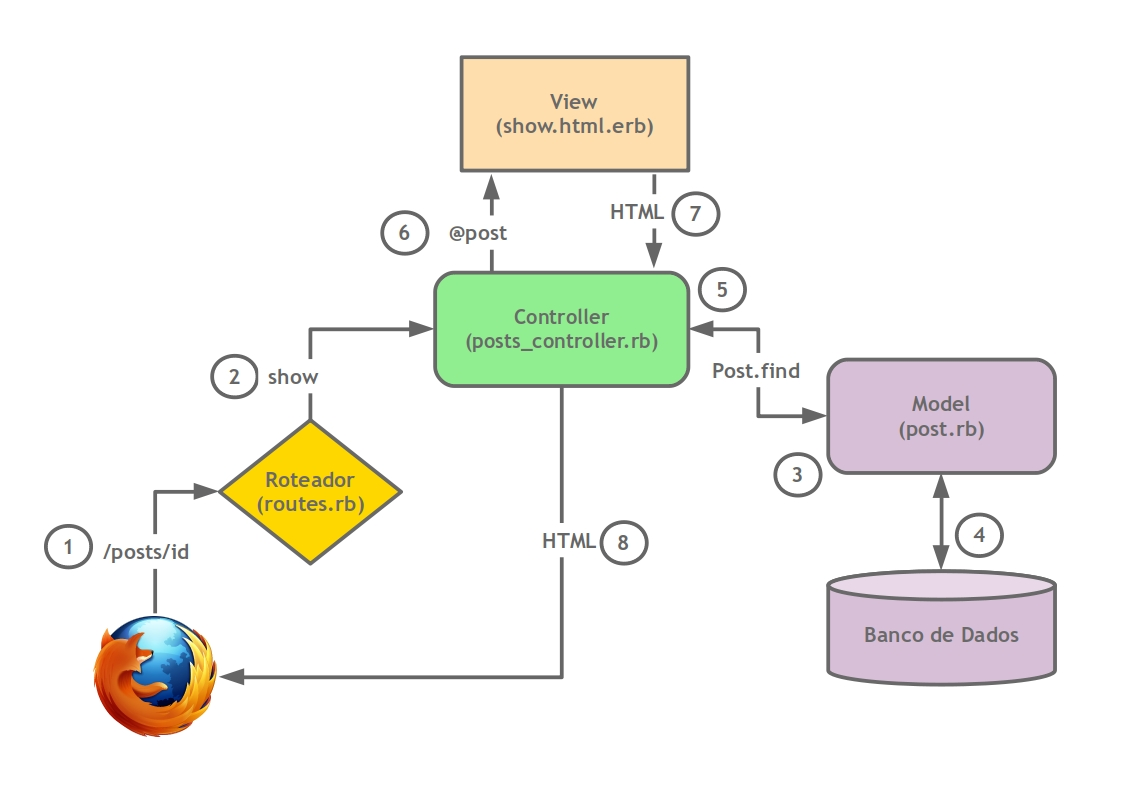
\includegraphics[width=0.75\textwidth]{imagens/mvc-action-show.jpg}
	\end{figure}
	\framebreak
	\begin{itemize}
		\item Recupera \alert{uma} postagem específica no parâmetro \alert{id} passado como parte da URL
		\item (Implicitamente) procura pelo \alert{show.html.erb} para renderizar a resposta
		\begin{lstlisting}[style=RubyInputStyle, caption=controllers/posts\_controller.rb]
class PostsController < ApplicationController
	def show 
		@post = Post.find(params[:id])
	end

	def new
		@post = Post.new
	end

	def create 
		@post = Post.new(post_params)
		
		@post.save
		redirect_to @post
	end
private 
	def post_params 
		params.require(:post).permit(:title, :body)
	end
end
		\end{lstlisting}
	\end{itemize}	
\end{frame}

%%-------------------------------------------------------------------------------------- Início
\begin{frame}[allowframebreaks, t, fragile]{Visão: Show}
	\begin{itemize}
		\item Implemente a visão \alert{show.html.erb}:
		\begin{lstlisting}[style=RubyInputStyle, caption=views/posts/show.html.erb]
<p>
	<strong>Title:</strong>
	<%= @post.title %>
</p>
<p>
<strong>Body:</strong>
	<%= @post.body %>
</p>
		\end{lstlisting}		
	\end{itemize}	
\end{frame}